%There are different classes of document, "article" is a useful one for scientific papers
\documentclass[letterpaper,11pt]{article}

%packages - these add different functionality, and there are many more
\usepackage{amsfonts}
\usepackage{graphicx}
\usepackage[left=2cm,top=2cm,right=2cm,bottom=1.5cm,head=.5cm,foot=.5cm]{geometry}
\usepackage{url}
\usepackage{multirow}
\usepackage{longtable}
\usepackage{subfig}
\usepackage{float}
\usepackage{setspace}
\usepackage{lineno}
\usepackage{natbib}
\usepackage{amsmath}
\usepackage{authblk}
\usepackage{xr}
\usepackage{relsize}
\usepackage{tikz}

%external documents - this lets you \ref labels defined in the SI, with the prefix SI-
\externaldocument[SI-]{LatexSimpleExample_SupMat}

%This is where the numeric results produced by the code get pulled in. The file
%NumericResults.tex is written by the code in ../code (code.R, code.py or code.m - it
%does not matter which, they all write the same file). It consists only of \newcommand
%lines, one per numeric result, so after this \input the macros \outputone (the slope)
%and \outputtwo (the intercept) are available to use anywhere in the text below. If
%you re-run the code and re-compile this document, the numbers in the pdf update
%automatically, with no copying and pasting. Nothing here depends on what language
%the code was written in.
\newcommand{\outputone}{1.959}
\newcommand{\outputtwo}{0.367}


%header material for paper delineated below but not actually run until \maketitle in the main document body
\title{A line fitted to ten points: a toy paper demonstrating a reproducible workflow}
\date{}

\author[a,b]{Pimsupa Jasmin Albert}
\author[a,*]{Daniel C. Reuman}

\affil[a]{Department of Ecology and Evolutionary Biology and Center for Ecological Research, University of Kansas}
\affil[b]{Environmental Studies Program and Department of Biology, University of Oregon}
\affil[*]{Corresponding author, reuman@ku.edu}

%This starts the actual body of the paper
\begin{document}

%adds linenumbers, good for submitting papers
\linenumbers

%actually creates the title, affiliations, etc in pdf
\maketitle

%The following is just to satisfy what the journal (Ecology Letters, in this case) wanted to see at the top
\noindent \textbf{Running head:} A line fitted to ten points \\
\noindent \textbf{Key words:} reproducibility, workflow, latex, linear regression, toy example \\
\noindent \textbf{Type of article:} Letter\\
\noindent \textbf{Words in Abstract:} 150; \textbf{Words in main text:} 4998; \textbf{Words in text boxes:} 0\\
\noindent \textbf{Number of references:} 40; \textbf{Number of figures:} 5; \textbf{Number of tables:} 1; \textbf{Number of text boxes:} 0\\
\noindent \textbf{Corresponding author:}
Daniel C. Reuman,
Department of Ecology and Evolutionary Biology,
University of Kansas,
2101 Constant Ave,
Lawrence, KS 66047;
Phone: 626-560-7084 \\
\noindent \textbf{Author emails:} pimsupaa@uoregon.edu, reuman@ku.edu\\
\noindent \textbf{Statement of Authorship:} The authors jointly carried out all parts of the study.\\
\noindent \textbf{Data accessibility statement:} All code and data for the project are available 
at \url{https://zenodo.org/record/8386993} and 
\url{https://github.com/jasminalbert/AsymmetricRelationshipsAndCoexistence}.

%Because the journal asked for it
\doublespacing

%This is how you do abstracts
\begin{abstract}
\noindent Fitting lines to points attracts wide 
interest in ecology. Etcetera.
\end{abstract}

%This is how you do sections, with labels for later citation
\section{Introduction}\label{section:introduction}

%How to just write text, and how to do a citation
At the core of ecology is the study of relationships between organisms and their environments.
If you don't believe that, check out \citep{Ghosh_2020_AER}. \cite{Ghosh_2020_AER} say some 
really convincing stuff. If you want to skip the parenthesis, use ``citealp", like this: \citealp{Ghosh_2020_AER}.

%How to cite a figure
To illustrate, the ten points in Fig. \ref{fig:toyline} appear to lie close to a straight line, 
and the line shown in Fig. \ref{fig:toyline} is the one we fitted to them. 

%Some math
Letting $N_i(t)$ denote the adult population density of species $i=1,2$ at time $t$, 
and defining $N = N_1(t)+N_2(t)$,
model equations are
\begin{equation}
N_i(t+1)=(1-\delta)N_i(t)+\delta N \frac{B_i(t)N_i(t)}{B_1(t)N_1(t)+B_2(t)N_2(t)}  \label{model_eq}
\end{equation}
for $i=1,2$. Here, $\delta$ is an adult mortality rate, and $B_i(t)$ is the fecundity of species $i$ at time $t$. 
The model postulates that adults die at rate $\delta$ at each time step, and are replaced by juveniles 
in proportion to the reproductive outputs of the species that year. Note that $N = N_1(t)+N_2(t)$ 
is constant. This model has nothing to do with the rest of this toy paper; it is here to show
what an equation looks like, and how to refer to one by number (it is equation \ref{model_eq}).

\section{Theory}\label{section:theory}

%This is how you cite another section by number
We here pursue goal G1: to fit a line to ten points. Go back and 
read the Introduction, which is section \ref{section:introduction}, if you are confused.

\section{Methods}\label{section:methods}

%More math - you can render ANY math you want. Find out when you need it. 
The model is 
\begin{equation}
y_i = \beta_0 + \beta_1 x_i + \epsilon_i, \label{line_eq}
\end{equation}
for $i=1,\ldots,10$, where $x_i=i$, the $y_i$ are the responses, $\beta_0$ is the intercept,
$\beta_1$ is the slope, and the $\epsilon_i$ are errors. The ``align'' environment lines up
several equations at the \& signs, like this:
\begin{align}
\hat{\beta}_1 &= \frac{\sum_i (x_i-\bar{x})(y_i-\bar{y})}{\sum_i (x_i-\bar{x})^2}, \\
\hat{\beta}_0 &= \bar{y}-\hat{\beta}_1 \bar{x}.
\end{align}
These are the ordinary least squares estimates of the parameters of equation \ref{line_eq}.

%How you cite an external document
See SI section \ref{SI-SIsect:reiter} for more details, and SI Fig. \ref{SI-fig:toylineSI} for 
the same figure again.

\section{Results}\label{section:results}

%How to include a numeric result without typing it. The macros \outputone and \outputtwo were
%defined by the \input in the preamble, and their values came from the code. One pitfall: a
%macro name eats the space that follows it, so "\outputone and" would print "1.959and". Using
%the macro inside math mode, as here, avoids the problem; outside math mode write \outputone{}
%with the empty braces, which ends the macro name without printing anything.
Our main result is that the fitted slope was $\hat{\beta}_1=\outputone$ and the fitted intercept 
was $\hat{\beta}_0=\outputtwo$ (Fig. \ref{fig:toyline}). Written out in words, the slope was 
\outputone{} and the intercept was \outputtwo{}, and if these look odd, remember the data were
made up. 

\section{Discussion}\label{section:discussion}

%This is how you do subsections. There is also a \subsubsection command, etc. 
\subsection{Discusion topic one}

Blah blah blah

\subsection{Discusion topic two}

More blah blah blah

\section{Author contributions}

Both authors contributed about equally to all parts of the paper.

\section{Acknowledgments}

The authors thank some people. 

\section{Funding information}

The authors were partly supported by some grants. 

%This is how you get it to use the Ecology Letters reference style. You can finds lots of such
%style files online for different journals. 
\bibliographystyle{ecology_letters2}
\bibliography{refs}

\clearpage
\newpage

%This is how you render a figure. The pdf comes straight from the results directory, where the
%code put it, so if the code changes the figure, the next compile of this document picks up the
%new version. (The subfig package, loaded above, is how you make multi-panel figures with
%(a), (b), (c) sub-captions; this toy figure has only one panel so it is not used here.)
\begin{figure}
%This part brings the pdf figure in
\centering
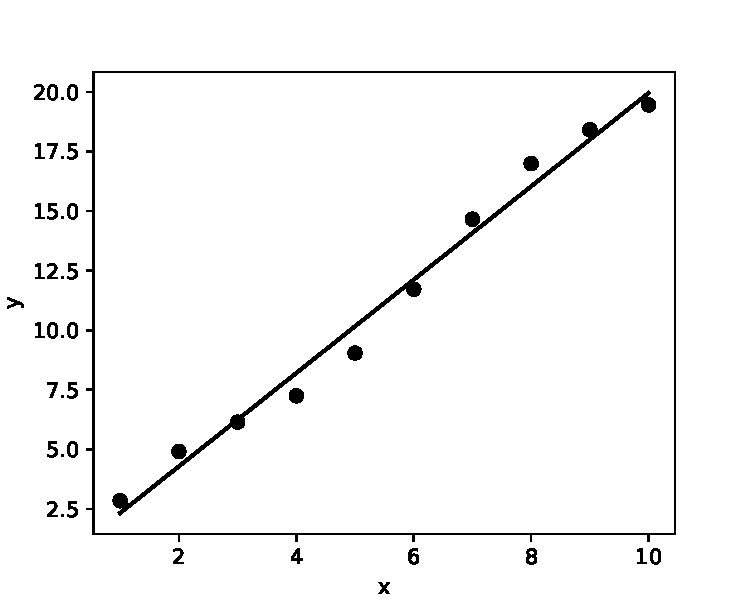
\includegraphics[width=0.6\textwidth]{../results/fig1.pdf}
%The caption. Note the numeric result can be used here too.
\caption{The ten toy data points (dots) and the line fitted to them by ordinary least squares
(solid line). The fitted slope was $\outputone$ and the fitted intercept was $\outputtwo$; see
section \ref{section:results}. Etcetera.
%This label is how you cite the figure
\label{fig:toyline}}
\end{figure}

\end{document}
